\documentclass[12pt,a4paper]{report}

% ---------------------------------------------------------------------------------
% Packages for Professional Academic Formatting
% ---------------------------------------------------------------------------------
\usepackage[a4paper,left=2.5cm,right=2cm,top=2.5cm,bottom=2.5cm]{geometry} % Standard margins
\usepackage{setspace}          % Line spacing
\usepackage[T1]{fontenc}       % Font encoding
\usepackage[utf8]{inputenc}    % Input encoding
\usepackage{titlesec}          % Heading formatting
\usepackage{tocloft}           % TOC formatting
\usepackage{graphicx}          % Images
\usepackage{hyperref}          % Hyperlinks
\usepackage{float}             % Figure positioning
\usepackage{listings}          % Code blocks
\usepackage{xcolor}            % Colors
\usepackage{caption}           % Captions
\usepackage{booktabs}          % Professional tables
\usepackage{enumitem}          % List formatting
\usepackage{microtype}         % Better justification and word spacing
\usepackage{indentfirst}       % Indent first paragraph after section
\usepackage{times}             % Times New Roman style font (standard for FYP)

% ----------------------------
% Document Global Settings
% ----------------------------
\onehalfspacing
\setlength{\parindent}{1.5em}  % Proper indentation
\setlength{\parskip}{0.5em}    % Spacing between paragraphs

% Prevent Widows and Orphans
\widowpenalty=10000
\clubpenalty=10000

% Heading Style Configuration
\titleformat{\chapter}[display]
  {\normalfont\huge\bfseries\centering}{\chaptertitlename\ \thechapter}{20pt}{\Huge}
\titlespacing*{\chapter}{0pt}{-20pt}{40pt}

\titleformat{\section}
  {\normalfont\Large\bfseries}{\thesection}{1em}{}
  
\titleformat{\subsection}
  {\normalfont\large\bfseries}{\thesubsection}{1em}{}

% List Style Configuration
\setlist[itemize]{leftmargin=2.5em, labelsep=0.5em, topsep=0pt, partopsep=0pt, itemsep=0.2em}
\setlist[enumerate]{leftmargin=2.5em, labelsep=0.5em, topsep=0pt, partopsep=0pt, itemsep=0.2em}

% ----------------------------
% Document Start
% ----------------------------
\begin{document}

% Front matter numbering
\pagenumbering{roman}

% ----------------------------
% Title Page
% ----------------------------
\begin{titlepage}
    \centering
    % Logo Placeholder
    % \includegraphics[width=4cm]{university_logo.png} 
    \vspace*{1cm}
    
    {\Large \textbf{FINAL YEAR PROJECT REPORT}\par}
    \vspace{1.5cm}
    
    {\Huge \textbf{BOTME: AI-POWERED PERSONALITY RECREATION PLATFORM}\par}
    \vspace{1.5cm}
    
    {\large Submitted By\par}
    \vspace{0.8cm}
    
    {\large
    \textbf{MALIK ALI HASSAN} (BSDSF21A011) \\
    \textbf{ALI HAMZA} (BSDSF22M032) \\
    \textbf{AHMED M. FAISAL} (BSDSF21A034) \\
    \textbf{MUNEEB AKRAM} (BSDSF21M061)
    \par}
    
    \vspace{1.5cm}
    
    {\large Supervised By\par}
    {\large \textbf{Mr./Ms. Supervisor Name}\par}
    {\large Designation (Assistant Professor)\par}
    
    \vfill
    
    {\large
    Submitted in partial fulfillment of the requirements for the degree of \\
    \textbf{Bachelor of Science in Data Science} \\
    (Session 2022--2026)
    \par}
    
    \vspace{1cm}
    
    {\large
    \textbf{DEPARTMENT OF COMPUTER SCIENCE} \\
    FACULTY OF COMPUTING \& INFORMATION TECHNOLOGY \\
    UNIVERSITY OF [UNIVERSITY NAME], [CITY]
    \par}
    
    \vspace{0.5cm}
    {\large \textbf{May 2026}}
    
\end{titlepage}

% ----------------------------
% Declaration
% ----------------------------
\chapter*{Declaration}
\addcontentsline{toc}{chapter}{Declaration}

We hereby declare that the project titled \textbf{“BOTME: AI-POWERED PERSONALITY RECREATION”} is our own work and has been developed responsibly. We confirm that:

\begin{itemize}
    \item This work has not been submitted previously for any degree or qualification in this or any other university.
    \item We have fully cited and referenced all external sources, libraries, and frameworks used in this project.
    \item We understand the university's policy on plagiarism and accept that any form of academic dishonesty will lead to the rejection of this project.
\end{itemize}

\vspace{2.5cm}

\begin{table}[h]
    \centering
    \begin{tabular}{p{6cm} p{1cm} p{6cm}}
        \textbf{Full Name} & & \textbf{Signature} \\[1.2cm]
        MALIK ALI HASSAN & & \rule{6cm}{0.4pt} \\[1.2cm]
        ALI HAMZA & & \rule{6cm}{0.4pt} \\[1.2cm]
        AHMED M. FAISAL & & \rule{6cm}{0.4pt} \\[1.2cm]
        MUNEEB AKRAM & & \rule{6cm}{0.4pt}
    \end{tabular}
\end{table}

\newpage

% ----------------------------
% Certificate of Approval
% ----------------------------
\chapter*{Certificate of Approval}
\addcontentsline{toc}{chapter}{Certificate of Approval}

This is to certify that the Final Year Project titled \textbf{“BOTME: AI-POWERED PERSONALITY RECREATION”} has been successfully completed by the students listed below under my supervision. 

The project is accepted in its present form as satisfying the requirements for the degree of \textbf{Bachelor of Science in Data Science}.

\vspace{1.5cm}

\textbf{Supervisor:} \\
\rule{7cm}{0.4pt} \\
\textbf{Mr./Ms. Supervisor Name} \\
Assistant Professor, Dept. of CS \\
University of [University Name]

\vspace{1.5cm}

\textbf{Internal Examiner:} \hfill \textbf{External Examiner:} \\
\rule{7cm}{0.4pt} \hfill \rule{7cm}{0.4pt} \\
Name: \hfill Name:

\vspace{1.5cm}

\textbf{Head of Department:} \\
\rule{7cm}{0.4pt} \\
Name: \\
Department of Computer Science

\newpage

% ----------------------------
% Executive Summary
% ----------------------------
\chapter*{Executive Summary}
\addcontentsline{toc}{chapter}{Executive Summary}

The BotMe system allows users to upload WhatsApp chat export files, which are then processed to create distinct AI personas. Leveraging Retrieval-Augmented Generation (RAG) technology, BotMe utilizes ChromaDB as a vector database to store and retrieve context-aware conversation fragments. This ensures that the AI remembers past interactions and responds in a manner consistent with the original user's style. 

Furthermore, the platform integrates advanced Voice Synthesis \& Text-to-Speech (TTS) capabilities using ElevenLabs API, allowing the AI personas to not only write but also speak in the cloned voice of the target individual. The platform is built on a robust tech stack featuring a React-based frontend for a modern interface and a Flask backend powered by LangChain, OpenAI's GPT-4o-mini, and ElevenLabs. Key features include automated personality analysis using the OCEAN model, high-fidelity voice cloning, and secure authentication via Google OAuth.

\newpage

% ----------------------------
% Acknowledgement
% ----------------------------
\chapter*{Acknowledgement}
\addcontentsline{toc}{chapter}{Acknowledgement}

We would like to express our sincere gratitude to our supervisor for their invaluable guidance, patience, and support throughout the development of this project. Their insights were instrumental in shaping the direction of BotMe and overcoming technical challenges.

We also thank the Faculty of Computing \& Information Technology for providing the necessary resources and an environment conducive to learning and innovation. A special thanks goes to our families and friends for their unwavering encouragement and understanding during long coding sessions and deadlines.

\vspace{3cm}

\begin{table}[h]
    \centering
    \begin{tabular}{p{6cm} p{1cm} p{6cm}}
        MALIK ALI HASSAN & & \rule{6cm}{0.4pt} \\[0.8cm]
        ALI HAMZA & & \rule{6cm}{0.4pt} \\[0.8cm]
        AHMED M. FAISAL & & \rule{6cm}{0.4pt} \\[0.8cm]
        MUNEEB AKRAM & & \rule{6cm}{0.4pt}
    \end{tabular}
\end{table}

\newpage

% ----------------------------
% Preliminaries
% ----------------------------
\tableofcontents
\newpage

\listoffigures
\newpage

\listoftables
\newpage

% ----------------------------
% Switch to Main Body Arabic Numbering
% ----------------------------
\pagenumbering{arabic}

% =================================================================================
% CHAPTER 1: INTRODUCTION
% =================================================================================
\chapter{Introduction}

\section{Background}
The advancement of Large Language Models (LLMs) has revolutionized the field of Artificial Intelligence, enabling machines to understand and generate human-like text with remarkable accuracy. However, most existing AI chatbots, such as ChatGPT or Gemini, operate as generic assistants. While they possess vast general knowledge, they lack the specific personal context, memories, and unique communication styles that define individual human interactions. Digital communication, particularly through platforms like WhatsApp, has become a primary medium for personal expression, creating rich archives of behavioral data that remain largely underutilized.

\section{Problem Statement}
There is a significant gap in the current AI landscape regarding personalization. Users today interact with "one-size-fits-all" AI models that cannot mimic specific individuals. This limitation becomes critical in scenarios such as digital legacy preservation, where families might wish to interact with a digital persona of a loved one. Furthermore, raw chat logs are unstructured and difficult to browse, making the valuable memories and personality traits buried within them inaccessible for interactive use.

\section{Proposed Solution}
BotMe proposes a web-based AI Persona Chatbot Platform that automates the conversion of unstructured WhatsApp chat data into interactive, memory-aware AI agents. By integrating Retrieval-Augmented Generation (RAG) with a vector database (ChromaDB), the system retrieves relevant past conversations to inform current responses, effectively simulating "memory." Additionally, the system incorporates Voice Synthesis \& Cloning, enabling the persona to generate spoken audio that mimics the original person's vocal characteristics.

\section{Objectives}
The primary objectives of the BotMe project are:
\begin{itemize}
    \item To develop a system that parses and processes WhatsApp chat export files (.txt) into structured data.
    \item To implement a RAG-based chatbot architecture that uses vector embeddings to maintain context.
    \item To integrate high-fidelity Voice Cloning and Text-to-Speech (TTS) technologies.
    \item To create a personality analysis module evaluating traits against the Big Five model.
    \item To build a secure, modern web application with role-based access control (Admin/User).
\end{itemize}

\section{Scope}
The scope of BotMe includes the development of a full-stack web application. The backend handles data processing and LLM interaction, while the frontend provides a responsive interface.

\textbf{In Scope:}
\begin{itemize}
    \item Text-based and Audio-based chat functionality.
    \item Interactive Voice Cloning using ElevenLabs.
    \item WhatsApp .txt file support.
    \item English/Roman Urdu language processing.
\end{itemize}

\section{Constraints}
\begin{itemize}
    \item \textbf{Data Privacy:} Chat logs contain sensitive personal information; the system ensures access control.
    \item \textbf{API Costs:} Reliance on OpenAI's API incurs costs based on token usage.
    \item \textbf{File Format:} Currently limited to standard WhatsApp export formats.
\end{itemize}

% =================================================================================
% CHAPTER 2: LITERATURE REVIEW
% =================================================================================
\chapter{Literature Review}

\section{Retrieval-Augmented Generation (RAG)}
RAG is a paradigm that enhances LLMs by retrieving relevant document chunks from an external knowledge base before generating a response. Unlike fine-tuning, which requires expensive retraining, RAG allows for dynamic knowledge updates. BotMe applies this concept to "personal memory," treating chat logs as the knowledge base.

\section{Personality Modeling in AI}
Personality computing involves the automated recognition and synthesis of human personality. The most widely accepted model is the Big Five (OCEAN: Openness, Conscientiousness, Extraversion, Agreeableness, Neuroticism). By analyzing a user's chat history, an AI can determine their personality profile and adjust its generation parameters accordingly.

\section{Comparison with Existing Systems}
\begin{table}[H]
\centering
\caption{Comparison of AI Chatbot Platforms}
\vspace{0.5em}
\begin{tabular}{@{}llll@{}}
\toprule
\textbf{Feature} & \textbf{ChatGPT} & \textbf{Character.AI} & \textbf{BotMe} \\ \midrule
Personal Context & Low (Session based) & Medium (Description) & High (Data based) \\
Data Source & Pre-training Data & User Manual Input & Actual Chat Logs \\
Memory Accuracy & Low & Medium & High (Vector) \\
Privacy & Public Model & Public Platform & Private/Secure \\ \bottomrule
\end{tabular}
\label{tab:comparison}
\end{table}

% =================================================================================
% CHAPTER 3: METHODOLOGY
% =================================================================================
\chapter{Methodology}

\section{Development Model}
BotMe was developed using the \textbf{Agile Methodology}. This iterative approach allowed for continuous improvement and feedback integration. The project was divided into sprints, focusing on delivering specific features such as the authentication module, chat parser, and RAG integration in sequential order.

\section{Tools \& Technologies Rationale}
\begin{enumerate}
    \item \textbf{React \& Vite:} Chosen for high performance and component reusability.
    \item \textbf{Flask:} A lightweight Python framework ideal for AI integration.
    \item \textbf{ChromaDB:} An AI-native vector database optimized for semantic search.
    \item \textbf{OpenAI GPT-4o-mini:} Selected for its high linguistic capability.
    \item \textbf{ElevenLabs:} Chosen for state-of-the-art Voice Cloning and Synthesis.
\end{enumerate}

% =================================================================================
% CHAPTER 4: SYSTEM DESIGN \& IMPLEMENTATION
% =================================================================================
\chapter{System Design \& Implementation}

\section{Overall System Architecture}
BotMe follows a modular Client-Server architecture. The Client is a Single Page Application (SPA), while the Server is a RESTful API serving as the bridge to AI services.

\begin{figure}[H]
    \centering
    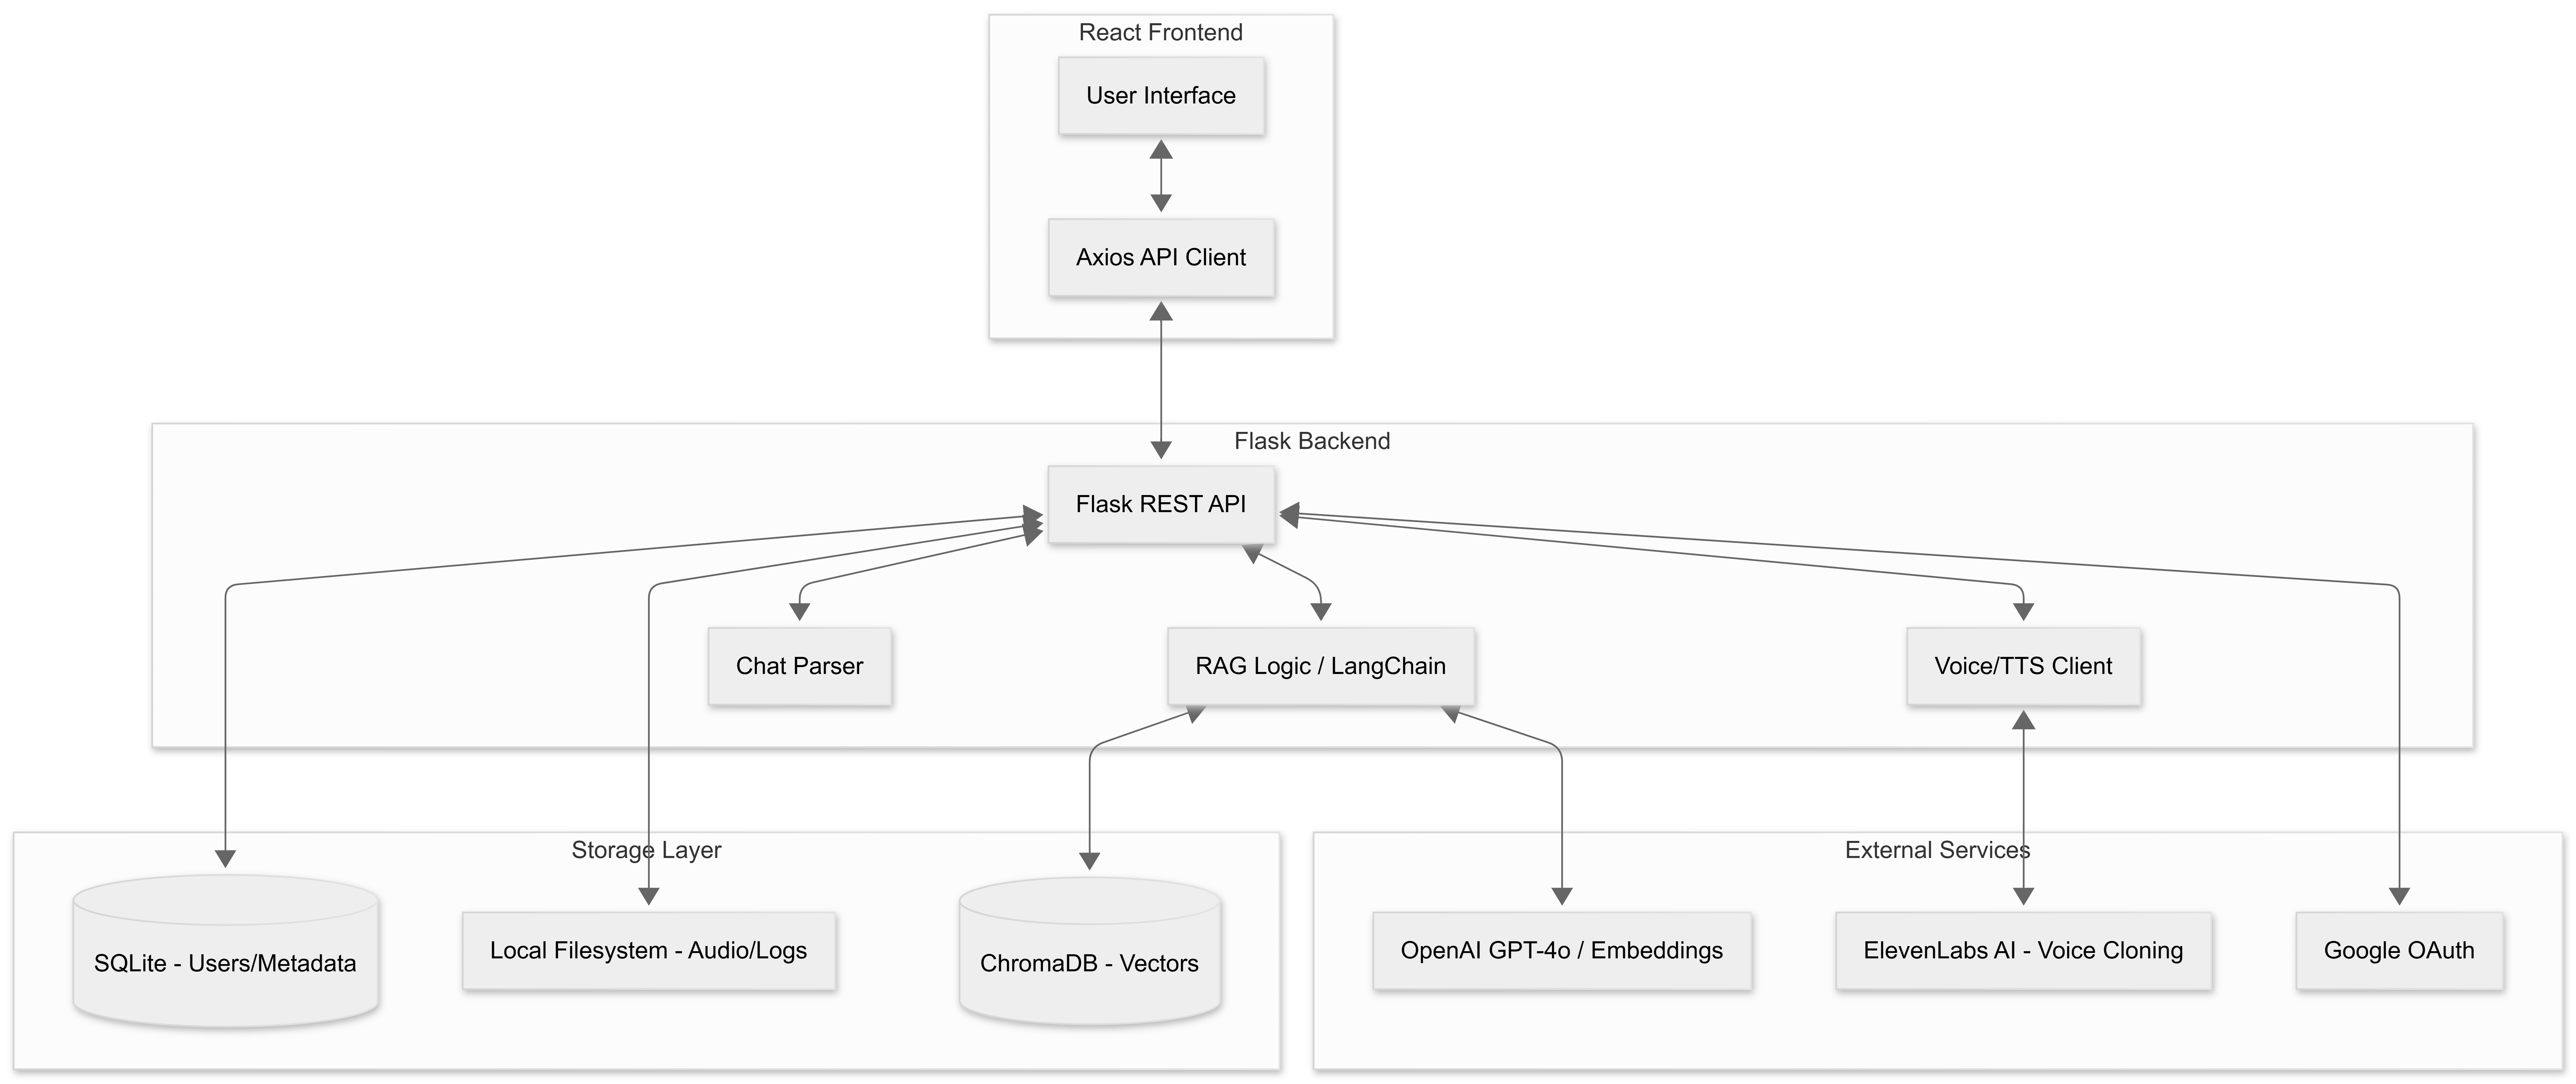
\includegraphics[width=0.8\textwidth]{System_Architecture.png}
    \caption{High-Level System Architecture}
    \label{fig:sys_arch}
\end{figure}

\section{System Workflow}
The workflow involves several key stages:
\begin{enumerate}
    \item \textbf{Authentication:} Secure entry via Email or Google OAuth.
    \item \textbf{Upload:} Processing WhatsApp \texttt{.txt} export files.
    \item \textbf{Parsing:} Cleaning and structuring dialogue by speaker.
\end{enumerate}

\begin{figure}[H]
    \centering
    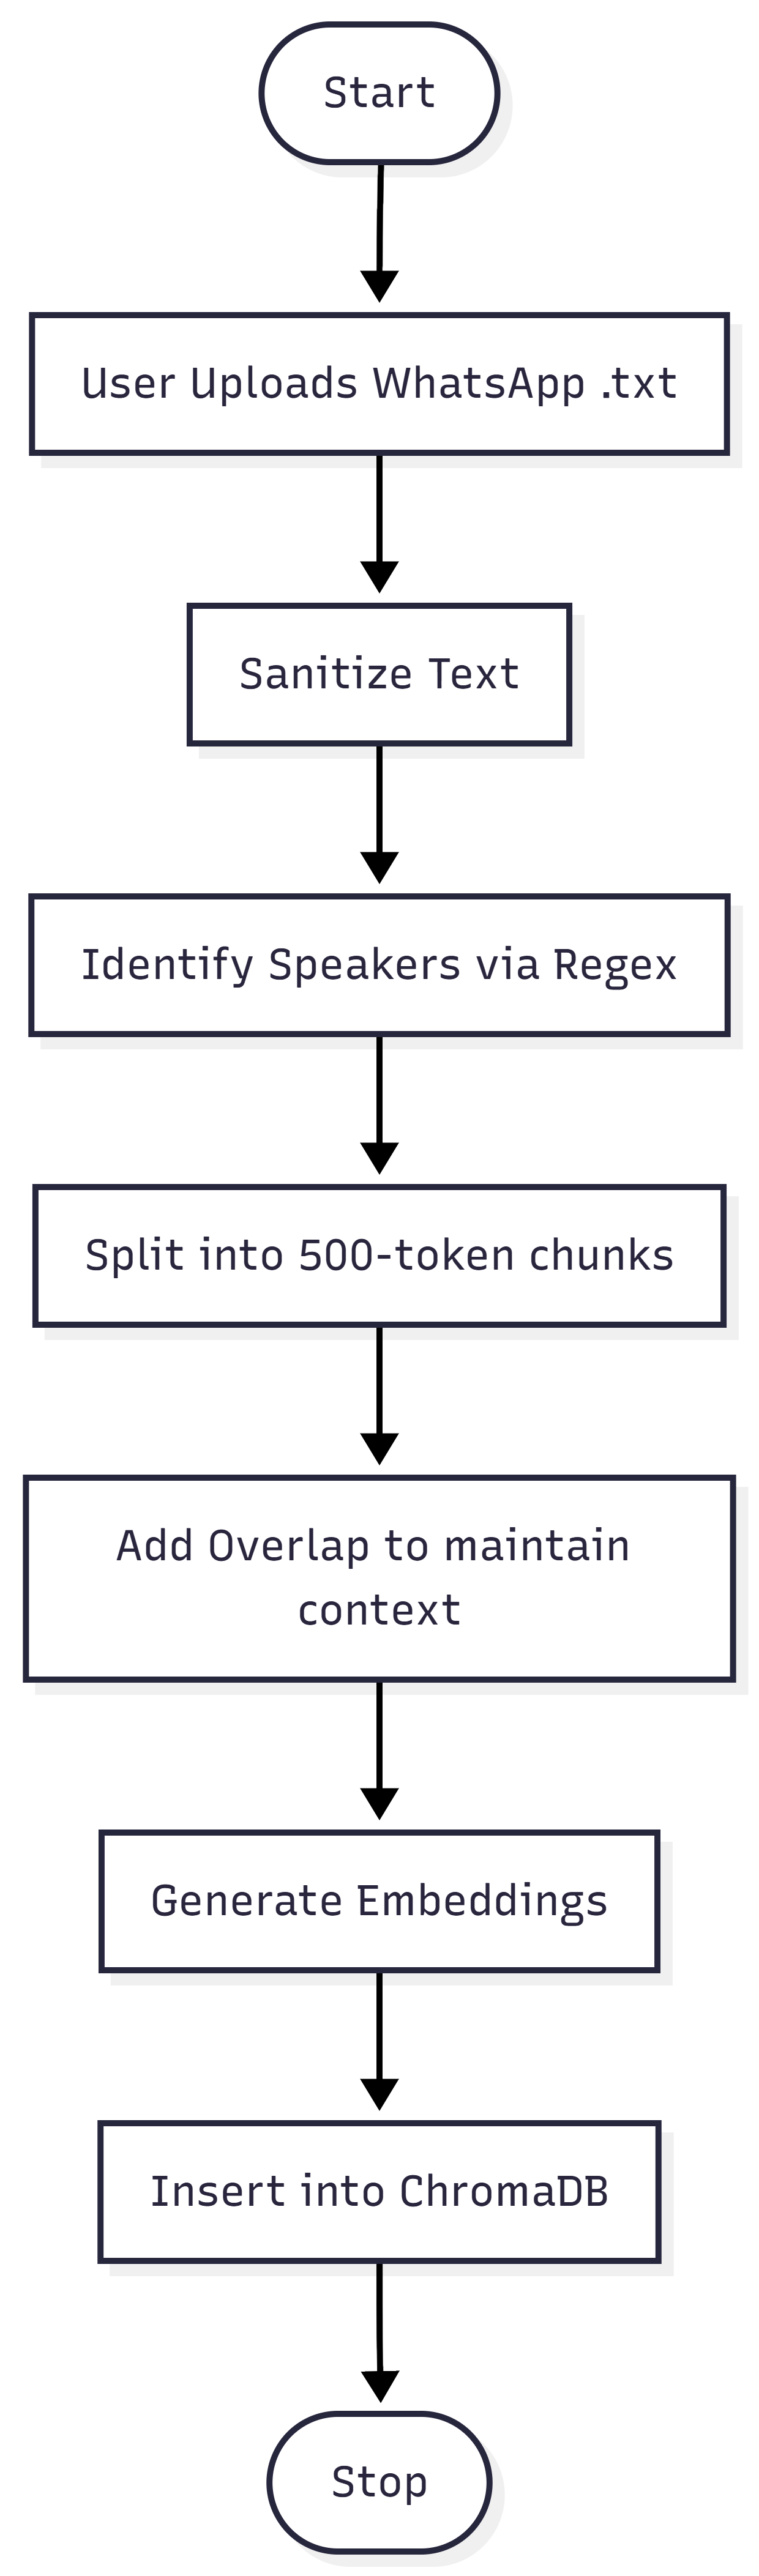
\includegraphics[width=0.8\textwidth]{DataIngestion.png}
    \caption{Data Ingestion Activity Diagram}
    \label{fig:data_ingestion}
\end{figure}

\begin{figure}[H]
    \centering
    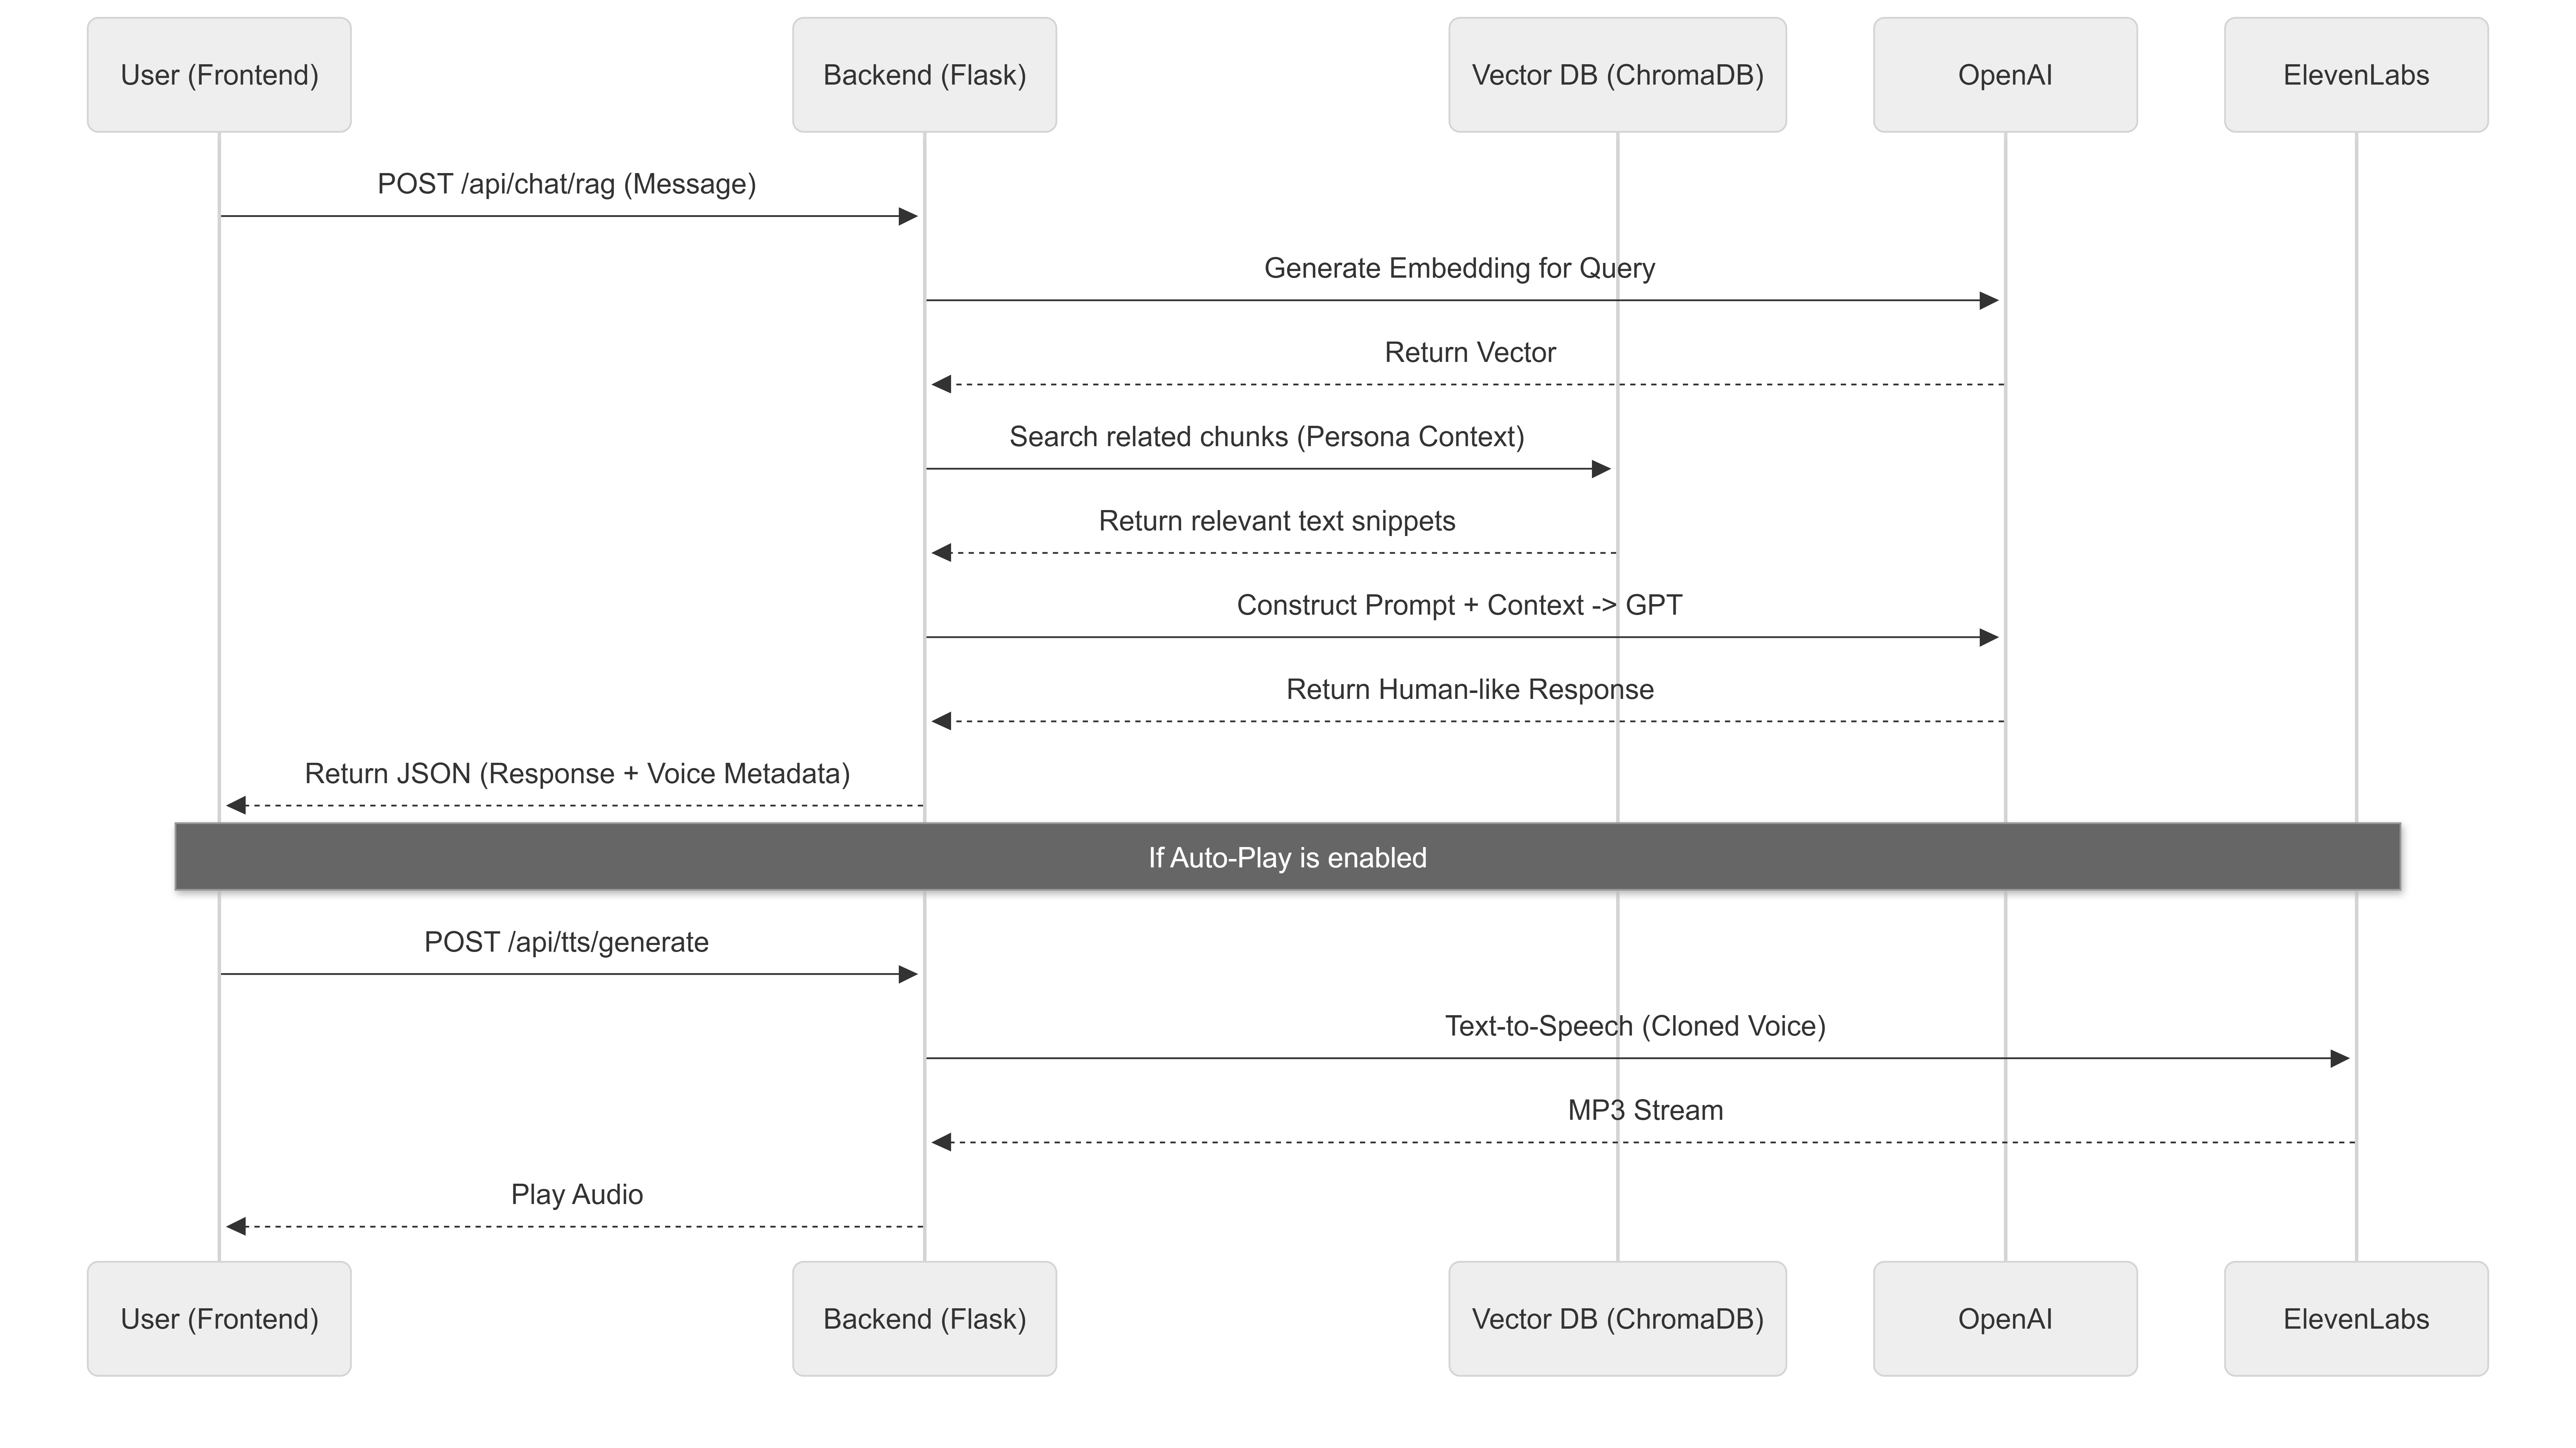
\includegraphics[width=0.8\textwidth]{Sequence.png}
    \caption{Chat Sequence Diagram: Message Processing}
    \label{fig:sequence}
\end{figure}

\section{Database Design}
The system uses a hybrid database approach:
\begin{itemize}
    \item \textbf{PostgreSQL (Relational):} Stores structured data such as Users and Personas.
    \item \textbf{ChromaDB (Vector):} Stores vector representations for semantic search.
\end{itemize}

\begin{figure}[H]
    \centering
    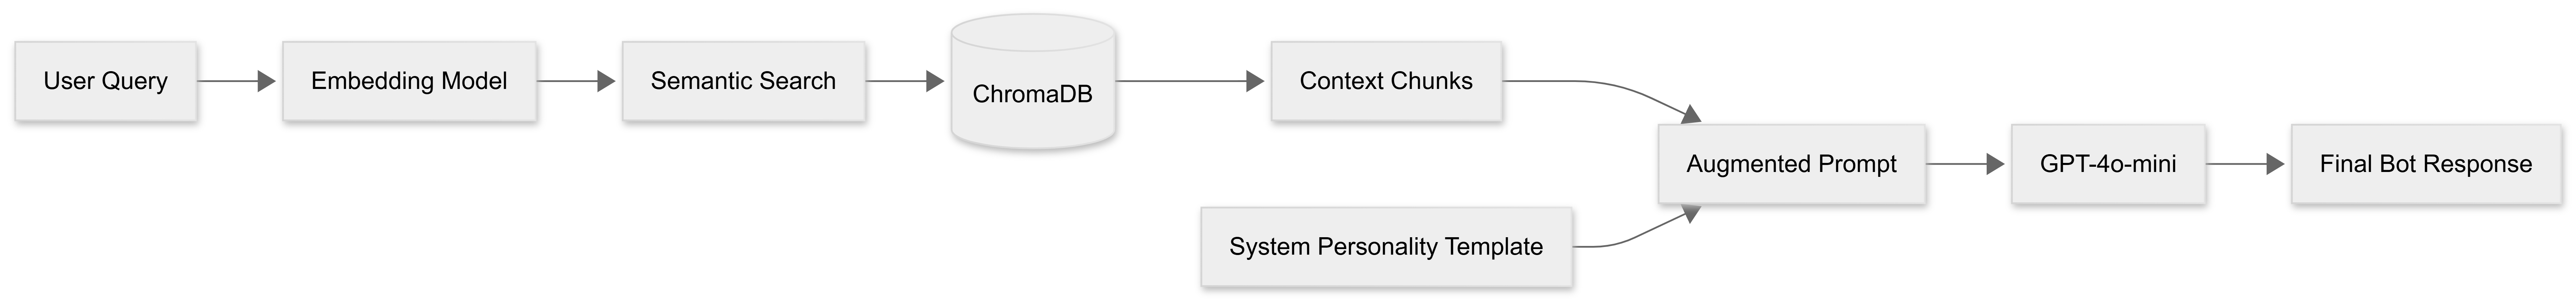
\includegraphics[width=0.8\textwidth]{RAG.png}
    \caption{RAG Logic Workflow}
    \label{fig:rag_flow}
\end{figure}

\begin{figure}[H]
    \centering
    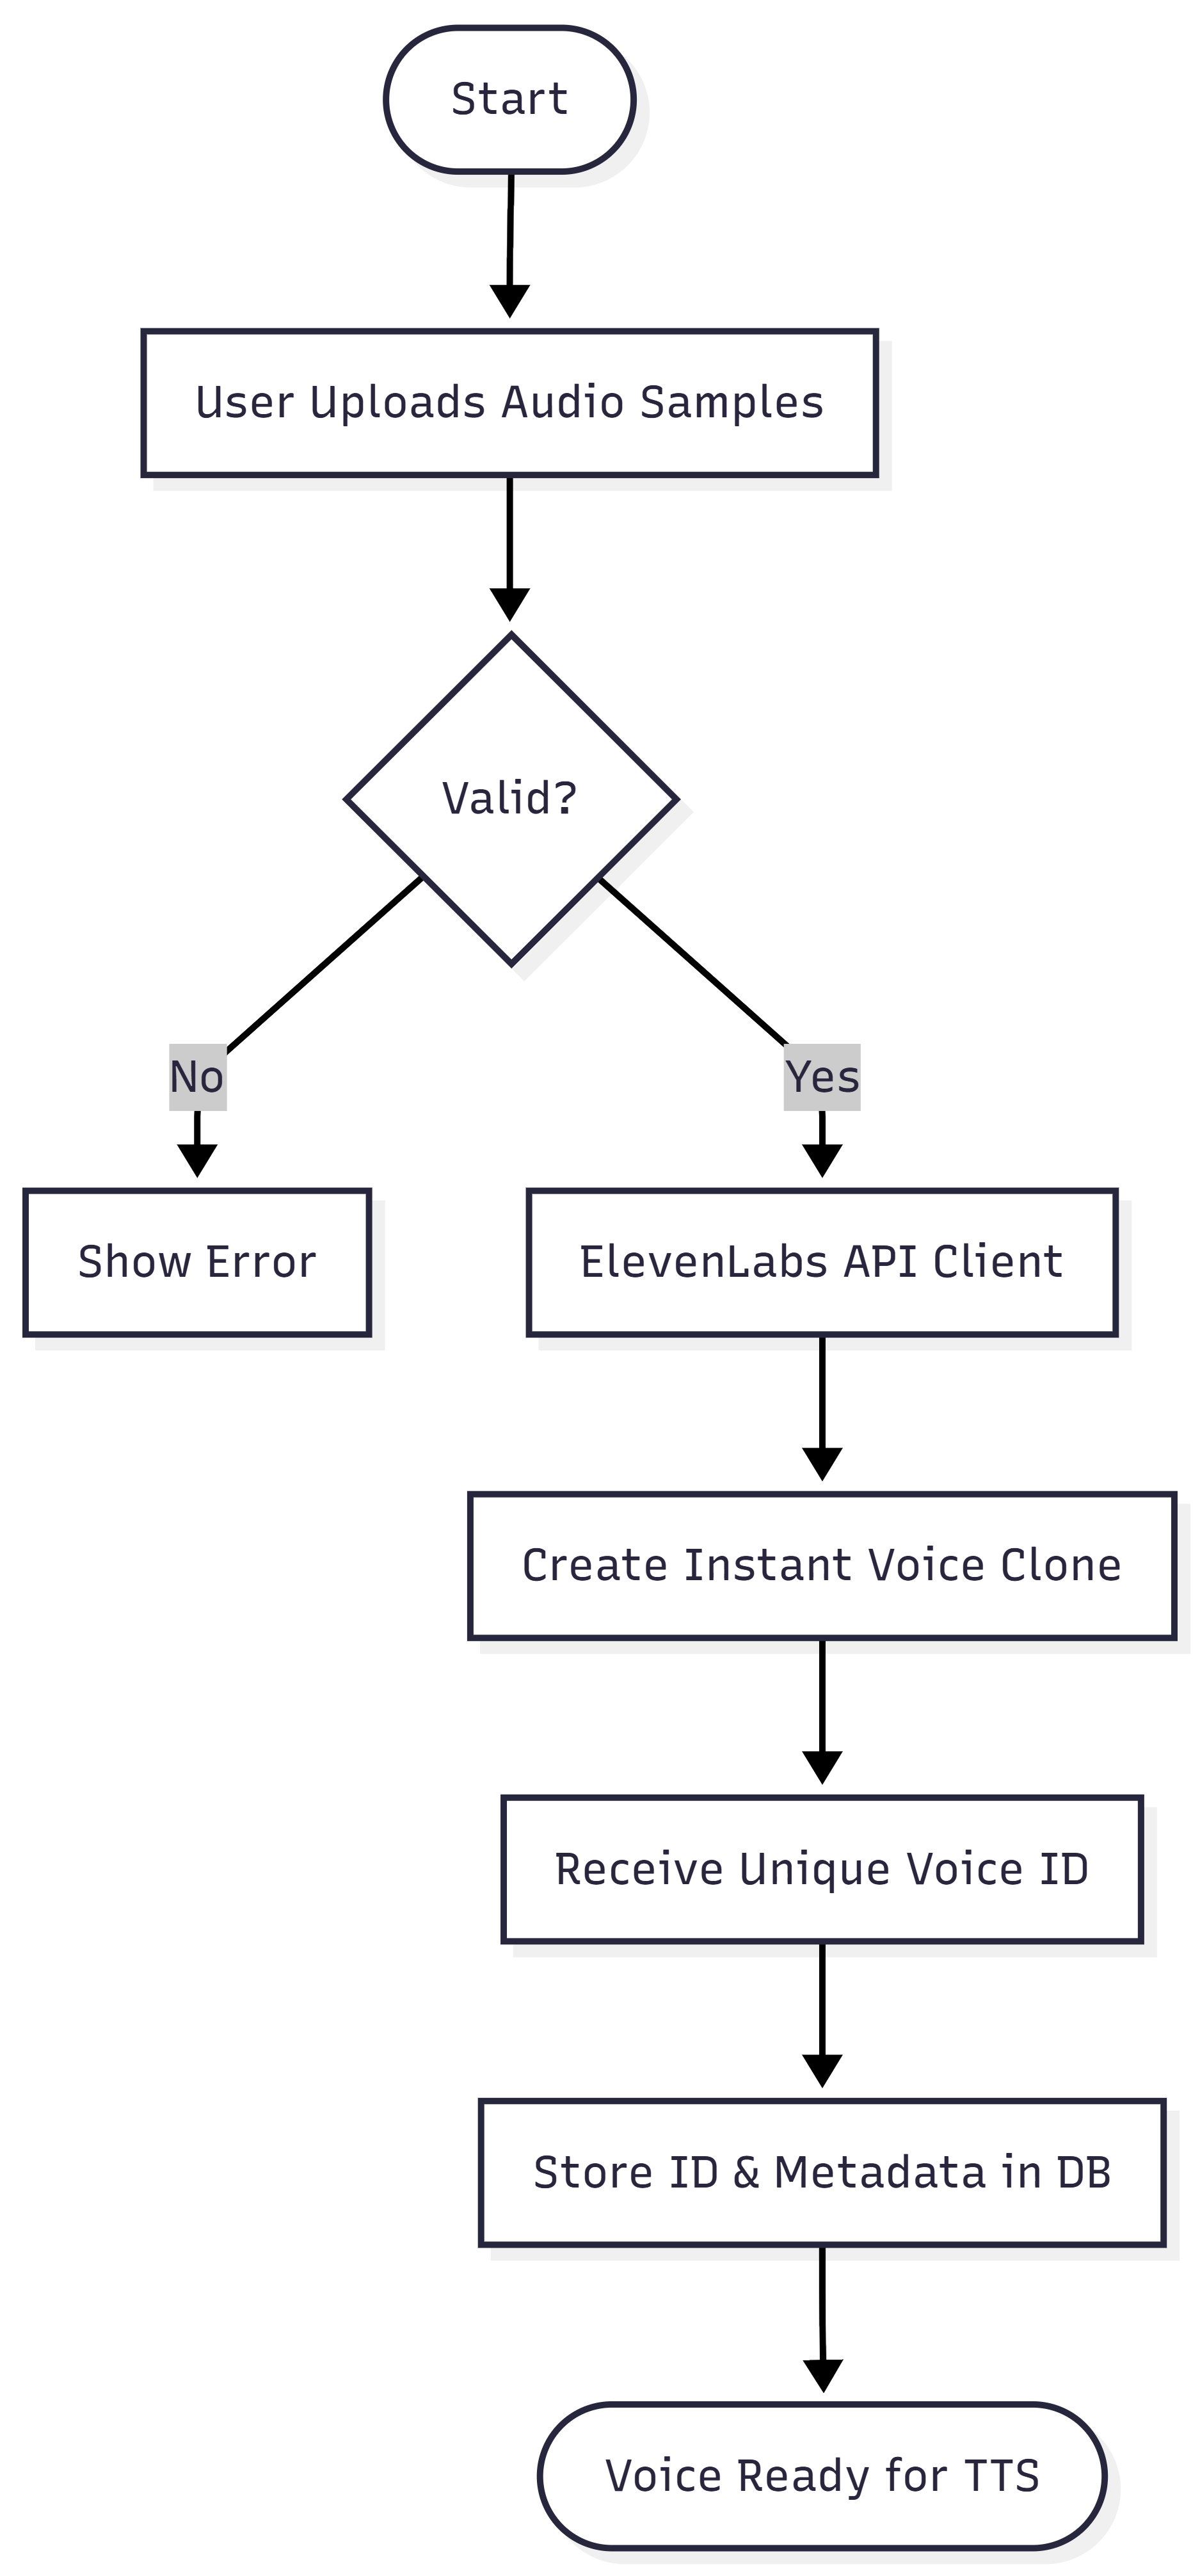
\includegraphics[width=0.8\textwidth]{Voice.png}
    \caption{Voice Cloning and TTS Integration Workflow}
    \label{fig:voice_cloning}
\end{figure}

% =================================================================================
% CHAPTER 5: RESULTS \& TESTING
% =================================================================================
\chapter{Results \& Testing}

\section{Test Cases}
\begin{table}[H]
\centering
\caption{System Test Cases and Results}
\vspace{0.5em}
\begin{tabular}{@{}lll@{}}
\toprule
\textbf{Test Case} & \textbf{Description} & \textbf{Outcome} \\ \midrule
TC-01: Upload & Upload 10MB WhatsApp .txt file. & Success (Parsed) \\
TC-02: Auth & Login with Google Account. & Success (Redirect) \\
TC-03: RAG & Ask about a past event. & Success (Context) \\
TC-04: Voice & Generate audio for persona. & Success (Match) \\ \bottomrule
\end{tabular}
\label{tab:testcases}
\end{table}

% \section{UI Screenshots Explanation}
% \textit{(Note: Screenshots to be included in final document layout)}
% \begin{itemize}
%     \item \textbf{Login Page:} Clean, minimal interface with "Sign in with Google" prominence.
%     \begin{figure}[H]
%         \centering
%         \includegraphics[width=0.8\textwidth]{login_page.png}
%         \caption{User Authentication Interface}
%         \label{fig:login_page}
%     \end{figure}
%     \item \textbf{Persona Dashboard:} A grid view of created personas with "Chat" and "Analyze" buttons.
%     \begin{figure}[H]
%         \centering
%         \includegraphics[width=0.8\textwidth]{dashboard.png}
%         \caption{Persona Management Dashboard}
%         \label{fig:dashboard}
%     \end{figure}
%     \item \textbf{Analysis View:} Radar charts prioritizing the visualization of Big Five personality traits.
%     \begin{figure}[H]
%         \centering
%         \includegraphics[width=0.8\textwidth]{personality_analysis.png}
%         \caption{Personality Analysis Visualization}
%         \label{fig:personality_analysis}
%     \end{figure}
%     \item \textbf{Chat Window:} Dark mode interface, distinguishing user messages (right) from bot messages (left).
%     \begin{figure}[H]
%         \centering
%         \includegraphics[width=0.8\textwidth]{chat_window.png}
%         \caption{Interactive Chat Interface with Voice Playback}
%         \label{fig:chat_window}
%     \end{figure}
% \end{itemize}

\section{Results Discussion}
The system successfully mimics the target persona in terms of tone and vocabulary. When presented with questions requiring specific knowledge, the RAG implementation consistently retrieves log entries that ground the AI's response in reality.

% =================================================================================
% CHAPTER 6: CONCLUSION & FUTURE WORK
% =================================================================================
\chapter{Conclusion \& Future Work}

\section{Achievements}
BotMe has successfully met its core objectives by delivering a functional platform that democratizes AI persona creation, secures user data, and demonstrates RAG implementation for hyper-personalization.

\section{Future Enhancements}
\begin{itemize}
    \item \textbf{Multi-modal Support:} Expanding beyond text to include image recognition.
    \item \textbf{Fine-Tuning:} Implementing LoRA techniques for higher linguistic fidelity.
    \item \textbf{Live Integration:} Real-time memory updates through browser extensions.
\end{itemize}

% ----------------------------
% References
% ----------------------------
\newpage
% \addcontentsline{toc}{chapter}{References}
\renewcommand{\bibname}{References}
\begin{thebibliography}{9}

\bibitem{rag2020}
P. Lewis et al., "Retrieval-Augmented Generation for Knowledge-Intensive NLP Tasks," in \textit{Proc. NeurIPS}, 2020.

\bibitem{ocean1992}
L. R. Goldberg, "The development of markers for the Big-Five factor structure," \textit{Psychological Assessment}, vol. 4, no. 1, 1992.

\bibitem{transformer2017}
A. Vaswani et al., "Attention Is All Need," in \textit{Proc. NIPS}, 2017.

\end{thebibliography}

\end{document}
